\subsection{Serviço de email -- VirtualIron}

O servidor de \emph{virtualização} utilizado neste caso é o Servidor \emph{VirtualIron}.

Os ficheiros de configuração deste serviço estão na localização por omissão. Para mais informações deverá consultar o manual do produto.

O conteúdo do servidor está localizado em:

\begin{Verbatim}
C:\Program Files\VirtualIron
\end{Verbatim}

O comando para controlar este serviço (iniciar/parar) é o seguinte:

\begin{figure}[H]
    \begin{center}
        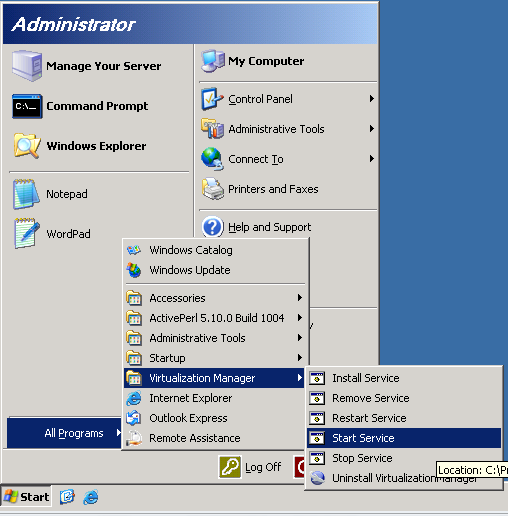
\includegraphics[width=10cm]{include/img/vi-win-start}
    \end{center}
    \caption{Iniciar o VirtualIron}
    \label{fig:VI-WIN1}
\end{figure}


\begin{figure}[H]
    \begin{center}
        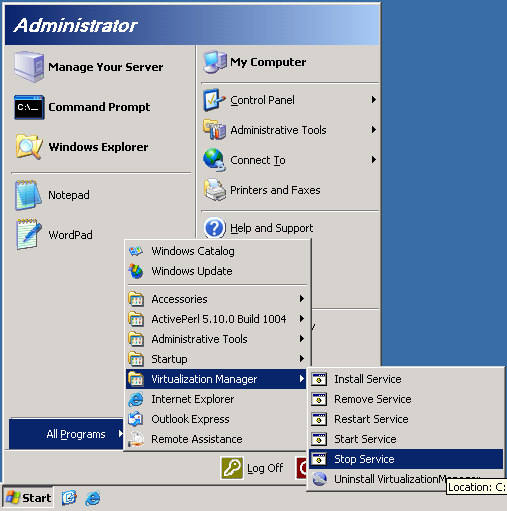
\includegraphics[width=10cm]{include/img/vi-win-stop}
    \end{center}
    \caption{Parar o VirtualIron}
    \label{fig:VI-WIN2}
\end{figure}



